\documentclass[12pt]{elsart}
\usepackage{amsmath}
\usepackage{amssymb}
\usepackage{program}
\usepackage{graphicx}
\usepackage[table]{xcolor}% http://ctan.org/pkg/xcolor
\newcommand{\field}[1]{\mathbb{#1}}

\usepackage{algorithm}
\usepackage{algpseudocode}

%%%%%%%%%%%%%%%%%%%%%%%%%%%%%%%%%%%%%%%%%Space to make more readable!
%\vspace{10 mm}
%%%%%%%%%%%%%%%%%%%%%%%%%%%%%%%%%%%%%%%%%Take out later!

\begin{document}

\pagestyle{empty}

\begin{center}
\Large  CS3343 Analysis of Algorithms Fall 2017 \\
\large {\bf Homework 5}\\
\normalsize Due 10/22/17 before 11:59pm (Central Time)
\end{center}

{\bf 1.  Hash Table Probabilities (3 points)}

\begin{enumerate}
   \item (1 point) Suppose $2$ keys are inserted into an empty hash table with $m$ slots. Assuming
simple uniform hashing, what is the probability of:
\begin{enumerate}
   \item exactly $0$ collisions occurring\\
      1 chance of no collision on first insertion and $(m - 1) / m$ chance on second insertion, so probability of 0 collisions is $\frac{m - 1}{m}$
   \item exactly $1$ collisions occurring\\
      1 chance of no collision on first insertion and $1 / m$ chance of only collision on second insertion, so probability of 1 collision is $\frac{1}{m}$\\
\end{enumerate}

   \item (2 points) Suppose $3$ keys are inserted into an empty hash table with $m$ slots. Assuming
simple uniform hashing, what is the probability of:
\begin{enumerate}
   \item exactly $0$ collisions occurring\\
      1 chance of no collision on first insertion, $(m - 1) / m$ chance on second insertion, and $(m - 2) / m$ on third insertion, so probability is $1 \cdot \frac{m - 1}{m} \cdot \frac{m - 2}{m} = \frac{m^2 - 3m + 2}{m^2}$
   \item exactly $1$ collisions occurring\\
      1 chance of no collision on first insertion, now two cases of only collision occurring, either on second or third insertion. Chance of collision on second and not on third is $1 \cdot \frac{1}{m} \cdot \frac{m - 2}{m} = \frac{m - 2}{m^2}$. Chance of collision on third but not on second is $1 \cdot \frac{m - 1}{m} \cdot \frac{2}{m} = \frac{2m - 2}{m^2}$. Total chance of 1 collision is $\frac{m - 2}{m^2} + \frac{2m - 2}{m^2} = \frac{3m - 4}{m^2}$
   \item exactly $2$ collisions occurring\\
      1 chance of no collision on first insertion, $1 / m$ chance of first collision on second insertion, and $2 / m$ chance of second collision on third insertion so probability of 2 collisions is $1 \cdot \frac{1}{m} \cdot \frac{2}{m} = \frac{2}{m^2}$
      
\end{enumerate}

\end{enumerate}


{\bf 2.  Red-Black Trees (2 points)}

\begin{enumerate}
\item Company X has created a new variant on red-black trees which also uses blue as a color for the nodes.  They call these ``red-black-blue trees".  Below are the new rules for these trees:\\

\begin{itemize}
   \item Every node is red, blue, or black.
   \item  The root is black.
   \item Every leaf (NIL) is black.
   \item If a node is red, then both its children are black.
   \item If a node is blue, then both its children are red or black.
   \item For each node, all simple paths from the node to descendant leaves contain the
same number of black nodes.\\
\end{itemize}

\begin{enumerate}
   \item (2 points) In class we found that the height, $h$, of a red-black tree is $\leq 2\log_2(n+1)$ (where $n$ is the number of keys).  Find and prove that a similar bound on height of the red-black-blue trees.
\\(Hint: You can use the same approach as we did to show\\ $h \leq 2\log_2(n+1)$).\\\\
      The number of nodes that are black on any simple path from the root to a leaf is at least $h / 3$ implied by property 4 and 5. It can be shown that a subtree rooted at any node $x$ contains at least $2^{bh(x)} - 1$ internal nodes. Using the root of the tree as $x$ we know that the number of nodes $n \geq 2^{h / 3} - 1 \rightarrow n + 1 \geq 2^{h / 3} \rightarrow \log_2(n + 1) \geq h / 3 \rightarrow 3\log_2(n + 1) \geq h$. Thus $h \leq 3\log_2(n+1)$\\

   \item (0 points - just for fun) Adding an additional color didn't seem to improve our bound on $h$ (i.e., 3 colors allows the tree to become more unbalanced than with 2 colors).    What benefit might we get from the extra color?\\
      Insertion would be easier and run in $O(1)$ time since it would only require a change in color to complete the insertion rather than $O(log(n))$
\end{enumerate}

\end{enumerate}

{\bf 3.  B-trees (4 points)}

\begin{enumerate}
   \item (2 points) Show the results of inserting the keys\\\\
$E,F,G,U,V,W,H$\\\\
in order into the B-tree shown below.  Assume this B-tree has minimum degree $k=2$. Draw only the configurations
of the tree just before some node(s) must split, and also draw the final configuration.
\newpage
\begin{figure}[h]
	\centering 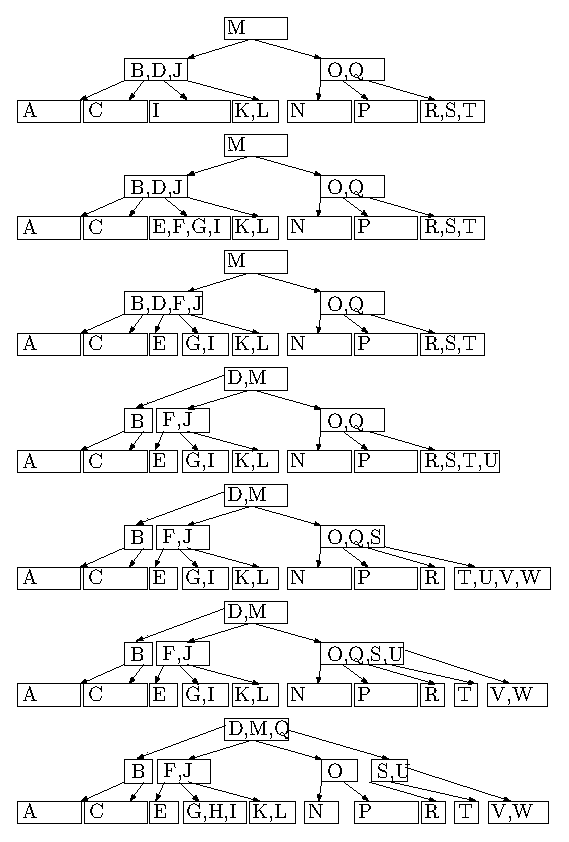
\includegraphics[width=0.7\textwidth]{BTreeProblem-01}
\end{figure}

   \item (2 points) Suppose you have a B-tree of height $h$ and minimum degree $k$. What is the largest number of keys that can be stored in such a B-tree?  Prove that your answer is correct.
\\(Hint: Your answer should depend on $k$ and $h$. This is similar to \\theorem we proved in the B-tree notes).\\
      \begin{tabular}{|l|l|l|}
        \hline
        level & num nodes & num keys\\
        \hline
        0 & 1 & $2k - 1$\\
        \hline
        1 & $2k$ & $2k(2k - 1)$\\
        \hline
        2 & $(2k)^2$ & $(2k)^2(2k - 1)$\\
        \hline
        \vdots & \vdots & \vdots\\
        \hline
        h & $(2k)^h$ & $(2k)^h(2k - 1)$\\
        \hline
      \end{tabular}\\
\newpage
      This table shows the maximum number of keys for a B-tree of degree $k$ and height $h$ at each given level. Summing the keys gives:\\
      \begin{flalign*}
        \sum\limits_{i=0}^{h} (2k)^i(2k - 1) &= (2k - 1)\sum\limits_{i=0}^{h} (2k)^i&\\
                                             &= (2k - 1) \frac{(2k)^{h+1} - 1}{2k - 1}\\
                                             &= (2k)^{h+1} - 1
      \end{flalign*}
      So the maximum number of keys in the given B-tree is $(2k)^{h+1} - 1$.
\end{enumerate}

{\bf 4.  Choose Function (4 points)}

Given $n$ and $k$ with $n \geq k \geq 0$, we want to compute the choose function ${n \choose k}$ using the following recurrence:

\hspace*{0.5cm} Base Cases: ${n \choose 0}=1$ and ${n \choose n}=1$, for $n\geq 0$\\
\hspace*{0.5cm} Recursive Case: ${n \choose k} = {n-1 \choose k-1} + {n-1 \choose k}$, for $n>k>0$

   \begin{enumerate}
      \item (1 point) Compute ${5 \choose 3}$ using the above recurrence.\\
          \begin{flalign*}
            {5 \choose 3} &= {4 \choose 2} + {4 \choose 3}&\\
                          &= {3 \choose 1} + {3 \choose 2} + {3 \choose 2} + {3 \choose 3}\\
                          &= {2 \choose 0} + {2 \choose 1} + {2 \choose 1} + {2 \choose 2} + {2 \choose 1} + {2 \choose 2} + 1\\
                          &= 1 + {1 \choose 0} + {1 \choose 1} + {1 \choose 0} + {1 \choose 1} + 1 + {1 \choose 0} + {1 \choose 1} + 1 + 1\\
                          &= 1 + 1 + 1 + 1 + 1 + 1 + 1 + 1 + 1 + 1\\
                          &= 10
          \end{flalign*}
\newpage
      \item (2 points) Give pseudo-code for a {\bf bottom-up} dynamic programming algorithm to compute ${n \choose k}$ using the above recurrence.\\
      \begin{algorithm}
        \caption{int choose(int $n$, int $k$)}
        \begin{algorithmic}[1]
        \State $C[n + 1][k + 1]$;
        \For{$i = 0$ {\bf to} $n$}
          \State $j = 0$;
          \While{$j \leq i$ {\bf and} $j \leq k$}
            \If{$j == 0$ {\bf or} $j == i$}
              \State $C[i][j] = 1$;
            \Else
              \State $C[i][j] = C[i - 1][j - 1] + C[i - 1][j]$;
            \EndIf
            \State $j++$;
          \EndWhile
        \EndFor
        \State return $C[n][k]$;
        \end{algorithmic}
      \end{algorithm}
      \item (1 point) Show the dynamic programming table your algorithm creates for ${5 \choose 3}$.

\begin{tabular}{ l||p{0.1\linewidth}|p{0.1\linewidth}|p{0.1\linewidth}|p{0.1\linewidth}|}
   & 0 & 1 & 2 & 3  \\
  \hline
  \hline
   0& 1 & \cellcolor{black!100} & \cellcolor{black!100}  & \cellcolor{black!100}\\
  \hline
   1& 1 & 1 & \cellcolor{black!100} & \cellcolor{black!100}\\
  \hline
   2& 1 & 2 & 1 & \cellcolor{black!100}\\
  \hline
   3& 1 & 3 & 3 & 1\\
  \hline
   4& 1 & 4 & 6 & 4\\
  \hline
   5& 1 & 5 & 10 & 10\\
  \hline
\end{tabular}
   \end{enumerate}

\end{document}